\documentclass[ngerman,math,12pt, t, dvipsnames, aspectratio=1610]{beamer}

\usepackage[T1]{fontenc}
%\usepackage[utf8]{inputenc}
\usepackage{babel}
\usepackage[scaled]{helvet}

\usetheme[math]{CAU2013b}

% fon
\usepackage{graphicx}
\usepackage[normalem]{ulem}
\usepackage{enumerate}
%\usepackage{microtype}
\usepackage{setspace}

% nur bei xetex
    \usepackage{fontspec} 
    %\usepackage[cm-default]{fontspec}
    \usepackage{xunicode}
    \usepackage{xltxtra}
    %\setmainfont{DejaVu Sans Condensed}
    %\setmainfont{FreeSerif}
    %\setsansfont{FreeSans}
    %\setmonofont{FreeMono}

% % % % Graphik    
    %\usepackage{fp}
    \usepackage{tikz}
    %\usepackage{xcolor}
    %% TikZ-Bibliotheken
    %\usetikzlibrary{arrows}
    %\usetikzlibrary{shapes}

% % Notizen
    %\usepackage{pgfpages}
    %\setbeameroption{show notes}
    %\setbeameroption{show notes on second screen=bottom}

% % % % Definitionen
\usepackage{thmbox}
%\newtheorem[L]{thmS}{Definition}  
\newtheorem{Def}{Definition}

% % % % Rahmen
\setlength{\fboxsep}{0pt}  % Rahmenabstand für Abbildungen

% % % % Code Listings
% % listings
%\usepackage{listings} % https://en.wikibooks.org/wiki/LaTeX/Source_Code_Listings
    %\lstset{ %
    %    basicstyle=\footnotesize,       % the size of the fonts that are used for the code
    %    showspaces=false,               % show spaces adding particular underscores
    %    showstringspaces=false,         % underline spaces within strings
    %    showtabs=false,                 % show tabs within strings adding particular underscores
    %    frame=single,                   % adds a frame around the code
    %    tabsize=4,                      % sets default tabsize to 2 spaces
    %    breaklines=true,                % sets automatic line breaking
    %    breakatwhitespace=false,        % sets if automatic breaks should only happen at whitespace
    %}

% % minted
    \usepackage{minted}      % für CodeFragmente
    \usemintedstyle{tango}
    \renewcommand*\familydefault{\sfdefault}

%
% % %
% % % % %
% % % % % % % %
% % % % % % % % % % % %
\title{xxxxTitel des Vortrages}
\subtitle{xxxxSubtitle}
\author{Oliver Nakoinz}
\institute{JMA}
%\date{2015-11-09}
\date{}

%% Handout: folgenden Block einkommentieren
%\usepackage{pgfpages}
%\pgfpagesuselayout{8 on 1}[a4paper, border shrink=5mm]
%\pgfpageslogicalpageoptions{1}{border code=\pgfusepath{stroke}}

%% Handout mit Notizen: folgenden Block einkommentieren
%%If you put the file  handoutWithNotes.sty either in your local texmf directory 
%%or in the same directory as your presentation you can include it with the following command
%\usepackage{pgfpages}
%\usepackage{handoutWithNotes}
%\pgfpagesuselayout{4 on 1 with notes}[a4paper,border shrink=5mm]
% % % % % % % % % % % % % %
% % % % % % %
% % %
%

\begin{document}
%\setbeamertemplate{background canvas}{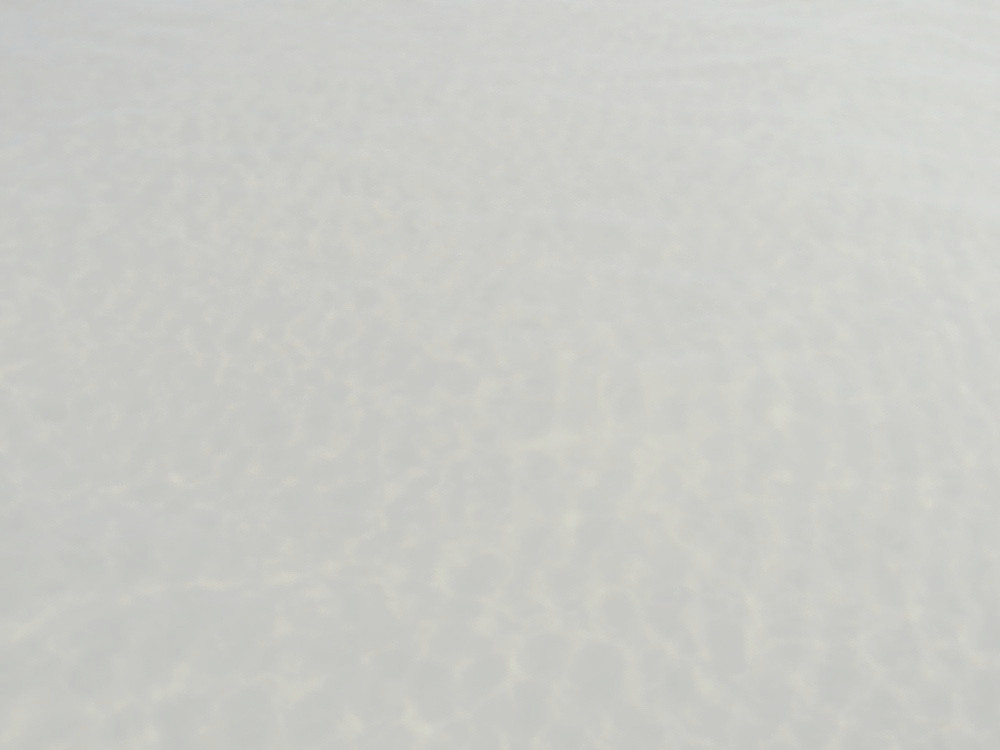
\includegraphics[width=1\paperwidth]{/home/fon/daten/bilder/hintergrund/hintergrund_fon_blass.JPG}}
\begin{frame}
    \vspace*{-2em}
    \titlepage  
    \vspace*{-2em}
    %\begin{center}
    %\textbf{Methods for Reconstructing Linear Structures of Monuments}
    %\end{center}
    
    \vspace*{-4em}
    \begin{columns}
        
        \column{.50\textwidth} \\
        \vspace*{2em}
        \hspace*{2em}
        %\tableofcontents[hideallsubsections] 
        \tableofcontents[currentsection]
        
        \column{.50\textwidth}\\
        \vspace*{2em}
        \hspace*{0em}
        %\fbox{\pgfimage[width=0.90\textwidth]{/home/fon/daten/bilder/karten/WOstsee2b.png}}\\
        
    \end{columns}
\end{frame}



\section{Einleitung}
\subsection*{slide xxxxxxxxxxxxxxxx}
\begin{frame}{Inhaltsbereichyyyyyyyyyyy}
  
Hier kommen Bilder etc hin und
Hier kommen Bilder etc hin und
Hier kommen Bilder etc hin und
Hier kommen Bilder etc hin und
Hier kommen Bilder etc hin und
Hier kommen Bilder etc hin und

\hrule

\end{frame}

\begin{frame}{Inhaltsbereich}{mit Untertitel}
\end{frame}
\end{document}
